\section{Modulationsarten}
Modulationsverfahren sind ein großes Anwendungsgebiet in der Nachrichtentechnik.
Ziel ist es viele Informationen Verlustfrei zu übertragen.
Möchte man ein Datensignal übertragen muss es davor
aufbereitet werden. Dies erledigt der Modulator/Mischer.
\\
Es gibt Analoge und Digitale Modulationsarten.
Für Analoge Signale werden folgende Verfahren verwendet.


\subsection{Amplitudenmodulation AM}
Die Idee hinter der Amplitudenmodulation ist dass das Informationssignal
auf die Amplitude des Trägersignals zu modulieren.
Daduch veränder sich die Amplituder des Trägersignals in abhängigkeit des Pegels und 
Freqeuenz des Informationssignals.
\\
\begin{figure}[h]
    \centering
    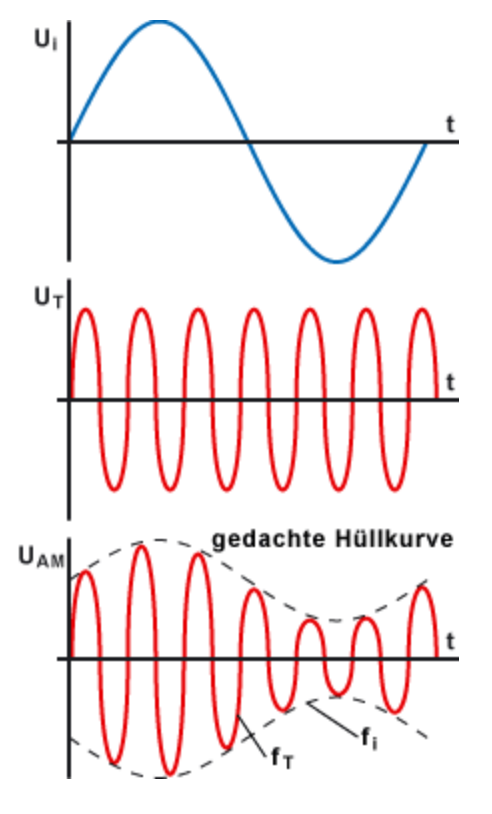
\includegraphics[width=0.22\textwidth]{Pictures/Screenshot 2025-06-19 125508.png}
    \caption{Amplitudenmodulation}
    \footnotesize{Quelle: \url{https://www.elektronik-kompendium.de/sites/kom/0401181.htm}}
    \label{fig:link_budget}
\end{figure}
\clearpage
Die Amplitude der Trägerschwingung wird durch das analoge Datensignal
$x(t)$ folgendermaßen verändert.
\begin{equation}
    a(t)=A_c(1+\mu x(t))
\end{equation}
Das AM-Signal wird beschrieben durch.
\begin{equation}
    x_c(t)=A_c(1+\mu x(t))cos(2\pi f_c t)
\end{equation}
\begin{itemize}
    \item $A_c$: Trägeramplitude
    \item $f_c$: Trägerfrequenz
    \item $\mu$: Modulationsindex 0 < $\mu$ < 1
\end{itemize}


\subsection{Frequenzmodulation FM}
Die Frequenzmodulation spielt eine eben so wichtige Rolle wie die Amplitudenmodulation,
ist im vergleich jedoch weniger Störanfällig. 
Hier wird auch ein hochfrequentes Trägersignal erzeugt und dadurch die Sendefrequenz um ein kleinen Betrag verändert.
Am einfachsten ist so eine Modulation durch ein LC-Schwingkreis.

\begin{equation}
x_c(t) = A_c \cos\left( 2\pi f_c t + 2\pi f_\Delta \int_0^t x(\tau) \, \mathrm{d}\tau \right)
\end{equation}
\begin{itemize}
    \item $x(\tau)$: Datensignal
    \item $A_c$: Amplitude des Trägersignals (konstant)
    \item $f_c$: Trägerfrequenz 
    \item $f_\Delta$: Frequenzhub, legt die maximale abwichung zu $f_c$ fest
\end{itemize}
\clearpage

\subsection{Phasenmodulation PM}
Die Phasenmodulation gehört wie die Frequenzmodulation zu den Winkelmodulationen.
Hier wird die Phase der Trägerwelle in Abhängigkeit des Datensignals verändert.
Die Phasenveränder bleibt im Signal erhalten variiert jedoch im vergleich
zur Ursprünglichen Phase des Trägersignal
\begin{figure}[h]
    \centering
    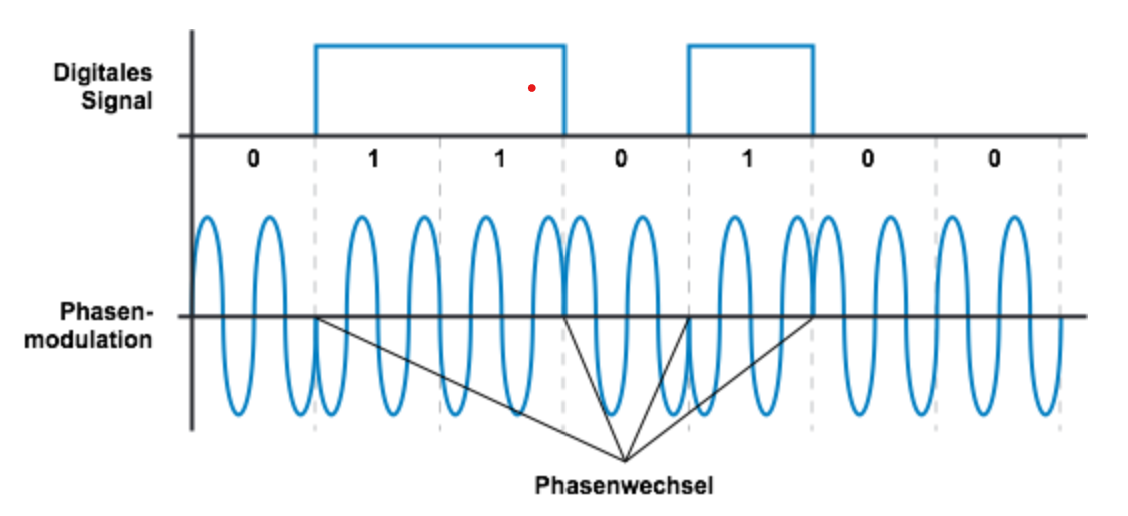
\includegraphics[width=0.5\textwidth]{Pictures/04020211.png}
    \caption{Phasenmodulation}
    \footnotesize{Quelle: \url{https://www.elektronik-kompendium.de/sites/kom/0402021.htm}}
\end{figure}

\section{Blockdiagramm einer Sendestrecke}
Im folgenden Abschnitt wird die Hochfrequenz-Übertragungsstrecke eines typischen Funksystems beschrieben. Bei der Abbildung 2.3 handelt es sich um ein Blockdiagramm. Es zielt darauf aus ein grundlegendes
systematisches Verständinis aufzubauen, um das gelernte auf unsere spezifische Hardware anwenden zu können. Die einzelnen Komponenten der Hochfrequenz-Übertragungsstrecke 
und deren Zusammenspiel wird im Anschluss näher erläutert und auf ihre Realiserung in unserer Hardware eingegangen.\\

\begin{figure}[h]
    \centering
    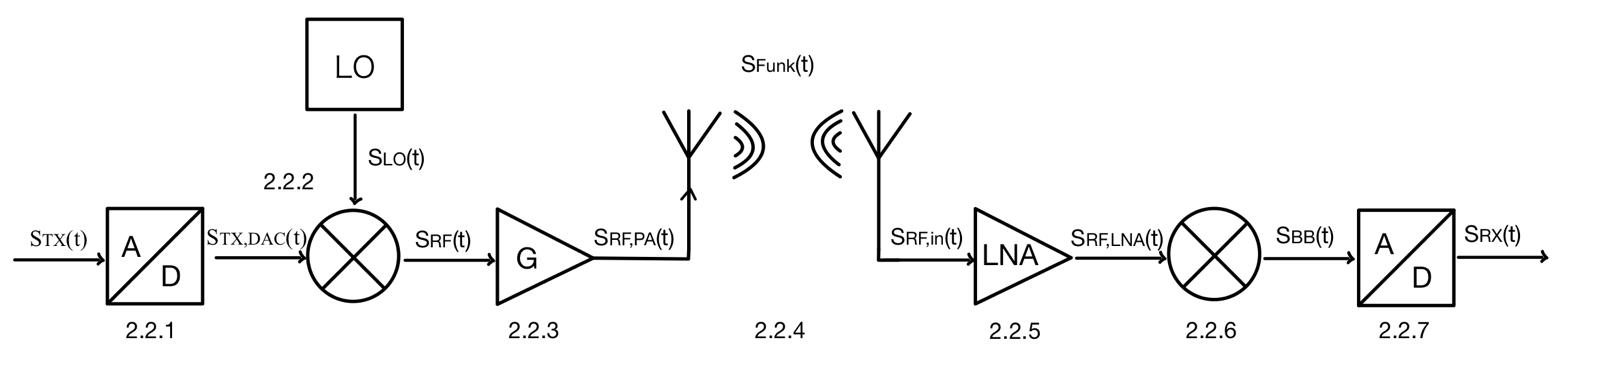
\includegraphics[width=1\textwidth]{Pictures/Blockdiagramm.jpg}   
    \caption{Blockdiagramm einer typischen Hochfrequenz-Übertragungsstrecke}
    %\footnotesize{Quelle: \url{https://www.elektronik-kompendium.de/sites/kom/0402021.htm}}
\end{figure}
\clearpage

\begin{minipage}{0.48\textwidth}
    \raggedright
    \textbf{\large Blockdiagramm-Komponente}\\[2ex]
    \begin{enumerate}
        \item [2.2.1] Digital-Analog-Wandler (DAC)
        \item [2.2.2] Lokaler Oszillator (LO)
        \item [2.2.2] Mischer: Modulator
        \item [2.2.3] Leistungsverstärker (PA)
        \item [2.2.4] Sende- und Empfangsantenne
        \item [2.2.5] Low Noise Amplifier (LNA)
        \item [2.2.6] Mischer: Demodulator
        \item [2.2.7] Analog-Digital-Wandler (ADC)
        
    \end{enumerate}
\end{minipage}%
\hfill
\begin{minipage}{0.48\textwidth}
    \raggedright
    \textbf{\large Funktion / Beschreibung}\\[2ex]
    \begin{itemize}
        \item $S_{\mathrm{TX}}(t)$: Digital erzeugtes Sendesignal
        \item $S_{\mathrm{TX;DAC}}(t)$: Analoges Signal (Basisbandsignal)
        \item $S_{\mathrm{LO}}(t)$: Sinusförmiges Trägersignal/ ungedämpfte hochfrequente Trägerschwingung
        \item $S_{\mathrm{RF}}(t)$: moduliertes analoges Hochfrequenzsignal
        \item $S_{\mathrm{RF,PA}}(t)$: Verstärkte Hochfrequenzsignal (durch PA)
        \item $S_{\mathrm{Funk}}(t)$: Signal auf Funkstrecke
        \item $S_{\mathrm{RF,in}}(t)$: Schwaches, empfangene Hochfrequenzsignal
        \item $S_{\mathrm{RF,LNA}}(t)$: Verstärkte Hochfrequenzsignal (durch LNA)
        \item $S_{\mathrm{BB}}(t)$: Demoduliertes analoges Basisbandsignal
        \item $S_{\mathrm{RX}}(t)$: Digitalisiertes Basisbandsignal
    \end{itemize}
\end{minipage}



\subsection{DAC}
Ein Digital-Analog-Wandler (eng. digital-to-analog converter, DAC) wandelt digitale Signale oder einzelne Werte in Analoge
Signale um. Bei einem digital Signal handelt es sich um ein zeit- und wertdiskretes Signal. Durch die Wandlung
in ein analoges Signal wird das Signal zeit- und wertkontinuierlich.  Dafür werden die Rechtecksignale des digitalen Eingangssignals mit Hilfe einer Fouriertransformation (evtl. Referenz zu theorie)
in eine  kontinuirlich veränderliche Spannung transfomiert. Diese Wandlung ist erforderlich um das Signal über eine
Antenne aussenden zu können, da Antennen nur elektormagnetische Wellen abstrahlen können. \\
Gehen wir nun auf unsere Hardware ein:
\\

\subsection{LO und Mischer}
Der lokale Oszillaotr(eng. local oscillator, LO) erzeugt eine ungedämpfte hochfrequente Trägerschwingung. Diese Trägerschwingung 
wird benötigt, um das analoge Signal auf die gewünschte Frequenz zu bringen. Der LO kann in verschiedenen Frequenzen arbeiten,
abhängig von der Anwendung und dem gewünschten Frequenzbereich des Signals. Der Mischer übernimmt die Modulation des
Bandsignals auf eine Hochfrequenz. Dies geschieht durch die Multiplikation des Bandsignals mit der Trägerschwinung des LO.
In unserer Schaltung ist der LO ein Quarz-Oszillator der bei einer Freqzenz $f=1,25GHz$ schwingt.

\begin{equation}
    S_{TX,DAC}(t) \cdot S_{LO}(t) \rightarrow S_{RF}(t)
\end{equation}


\subsection{PA}
Der Leistungsverstärker (eng. power amplifier, PA) verstärkt das modulierte Signal auf eine Leistung, die für die Übertragung über eine Antenne 
geeignet ist. Die hohe Leistung ist notwedig um über eine größere Diszanz senden zu können und um Zuverlässigkeit und
Signalqualität zu gewährleisten. 

\subsection{Drahtlose Übertragung mit Antennen}
Die Sendeantenne strahlt das modulierte HF Signal Sxx als elektromagnetische Wellen in den Raum ab. DIese abgstrahlte Welle
breitet sich mit Lichtgeschwindigkeit aus und kann von Empfängerantennen empfangen werden. Die Empfängerantenne wandelt
die elektromagnetische welle wieder in eine elektrische Spannung um, die dann weiterverarbeitet werden kann. Diese entspricht
jedoch nicht mehr dem ursprünglichen Bandsignal, da es durch die Übertragungseinflüsse wie Dämpfung, Rauschen und Interferenzen
und vielen weiteren Einflüssen gedämpft und gestört wurde.

\subsection{LNA}
Bei dem LNA (eng. low noise amplifier) handelt es sich um einen rauscharmen HF-Verstärker. Das empfangene Signal Sxx ist
durch die bereits erwähnten Einflüsse sehr schwach und muss  zuerst verstärkt werden, um weiterverarbeitet werden. Daher
ist eine Verstärkung des Signals unmittlbar nach der Antennen zwingend notwendig. Der Vorteil des LNA gegenüber zu
anderen Verstärkern ist, dass er kein nennenswertes Rauschen hiinzufügt. Dies ist wichtig, da jedes zusätzliche Rauschen
die folgende Demolution erheblich erschweren würde. Ebenfall ist durch die Postion des LNA das empfangene Signal noch 
nicht durch andere elektrischen Komponenten verfälscht worden, was durch eine spätere Verstärkung zu rekonstruktionsproblemen
des eigentlichen Signals führen könnte.
\subsection{Demodulation}
Die Demodulation ist der Prozess, bei dem das modulierte Signal wieder in das ursprüngliche Bandsignal zurücgewandelt wird. Dieser Schritt erfolgt
vor dem ADC weil die Frequenz des Hochfrequenzsignals zu hoch ist um es direkt mit einem üblichen ADC zu digitalisieren. Die dafür notwendige
Abtastrate wöre hierbei extrem hoch.
Das Nyquist-Abtasttheorem besagt, dass ein Signal der maximalen Frequenz $f_\mathrm{max}$ nur dann verlustfrei rekonstruiert werden kann,
wenn die Abtastfrequenz $f_\mathrm{s}$ mindestens doppelt so groß ist wie $f_\mathrm{max}$:
\begin{equation}
    f_\mathrm{s} \geq 2 f_\mathrm{max}
\end{equation}
(Samplerate richtig? Die Trägerfrequenz unseres
Modulators beträgt $f=1,25GHz$. Das würde mindestens 2,5 Gigasamples pro Sekunde erfordern.) ADC die in der Lage sind solch hohe Frequenzen
zu verarbeiten sind kosten-, energie- und datenintensiv. -> Nicht für unser Praktikum geeignet wegen spaaaaaren xD.\\
\\
Schwierigerer Teil. CGPT cooken lassen (irgendwie schaltplan einfügen, nummern von andric genommen). Betrachten wir nun die Koversion 
(=Frequenzumsetzung) vom HF-Signal in ein digitales Nutzsignal im Empfänger in unserer Schaltung. 



\subsection{ADC}
Nun muss das demodulisierte Signal wieder in ein digitales Signal umgewandelt werden, damit es weiterverarbeitet werden kann.
In unsere Schaltung wird dafür ... verwendet. 


\section{Mathematische Grundlagen: Fourier-Transformation}
\subsection{Betrag und zeitlicher Verlauf von Rechteckfunktion}
Der Rechteckimpuls ist eine wichtige Funktion in der Signalverarbeitung.
Er wird häufig in der Kommunikationstechnik verwendet, um digitale Signale zu repräsentieren.
Der Verlauf der Rechteckfunktion $x(t)$ ist in Abbildung \ref{fig:rechteck} dargestellt.
\begin{figure}[H]
    \centering
    \begin{tikzpicture}
        \begin{axis}[
            width=0.8\textwidth,
            height=5cm,
            axis lines=middle,
            xlabel={$t$},
            ylabel={$x(t)$},
            domain=-2:2,
            samples=200,
            xtick={-2,-1,0,1,2},
            ytick={0,1},
            ymin=-0.2, ymax=1.2,
            grid=both,
        ]
        % Null-Linie links
        \addplot[blue, thick, samples=2, domain=-2:-1] {0};
        % Rechteck oben
        \addplot[blue, thick, samples=2, domain=-1:1] {1};
        % Null-Linie rechts
        \addplot[blue, thick, samples=2, domain=1:2] {0};
        % Vertikale Linie bei t=-1
        \addplot[blue, thick, samples=2, domain=0:1] ({-1},{x});
        % Vertikale Linie bei t=1
        \addplot[blue, thick, samples=2, domain=0:1] ({1},{x});
        \end{axis}
    \end{tikzpicture}
    \caption{Verlauf der Rechteckfunktion $x(t)$ mit Amplitude 1 im Intervall $-1 < t < 1$}
    \label{fig:rechteck}
\end{figure}

Die Rechteckfunktion $x(t)$ ist gegeben durch:
\[
x(t) = \begin{cases}
    1 & \text{für } -1 < t < 1 \\
    0 & \text{sonst}
    \end{cases}
\]
    
Die Fourier-Transformierte einer Rechteckfunktion der Breite $2T$ und Höhe $1$ ist gegeben durch die normierte $\mathrm{sinc}$-Funktion:
\[
\mathcal{F}\{x(t)\} = 2T \cdot \mathrm{sinc}(T\omega) = 2T \cdot \frac{\sin(T\omega)}{T\omega}
\]
Der Verlauf der Fourier-Transformierten ist in folgender Abbildung dargestellt:

\begin{figure}[H]
    \centering
    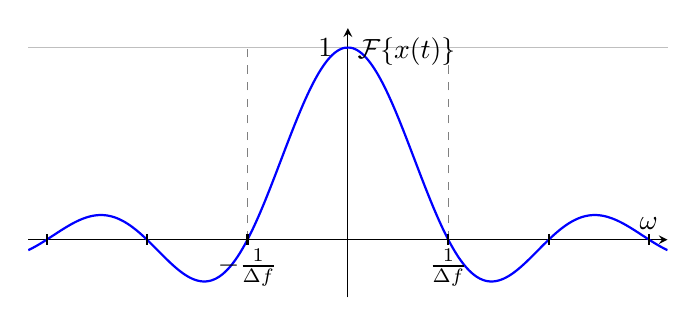
\begin{tikzpicture}
        \begin{axis} [
            width=0.8\textwidth,
            height=5cm,
            axis lines=middle,
            xlabel={$\omega$},
            ylabel={$\mathcal{F}\{x(t)\}$},
            domain=-10:10,
            samples=400,
            xtick=\empty, % entfernt die Zahlen auf der x-Achse
            ytick={-1,0,1},
            ymin=-0.3, ymax=1.1,
            grid=both,
        ]
        \addplot[blue, thick, samples=400, domain=-10:10] {sin(deg(x))/x};
        % Markiere die Nullstellen bei x = -pi und x = pi (entspricht ±1/Δf)
        \draw[dashed,gray] (axis cs:-3.1416,0) -- (axis cs:-3.1416,1);
        \draw[dashed,gray] (axis cs:3.1416,0) -- (axis cs:3.1416,1);
        \node[below] at (axis cs:-3.1416,0) {$-\frac{1}{\Delta f}$};
        \node[below] at (axis cs:3.1416,0) {$\frac{1}{\Delta f}$};
        % Einfache Striche für Vielfache von 1/Delta f
        \foreach \k in {-3,-2,-1,1,2,3} {
            \addplot[black, thick, mark=none, domain=0:0.03, samples=2] coordinates {({\k*3.1416},0.03) ({\k*3.1416},-0.03)};
        }
        % Optional: Nullstelle bei 0 markieren (falls gewünscht)
        % \addplot[black, thick, mark=none, domain=0:0.03, samples=2] coordinates {(0,0.03) (0,-0.03)};
        \end{axis}
    \end{tikzpicture}
    \caption{Verlauf der Fourier-Transformierten der Rechteckfunktion: $\mathrm{sinc}(\omega)$, Nullstellen bei Vielfachen von $\frac{1}{\Delta f}$}
    \label{fig:fourier_rechteck}
\end{figure}

Die Rechteckfunktion ist in der digitalen Signalverarbeitung von Relevanz, da diese eine Basis für die Änderung des Signalpegels darstellt. Durch die Idealisierung lässt sich der High-Pegel (1) und Low-Pegel (0) des Signals gut darstellen. In der Praxis wird die Rechteckfunktion jedoch durch eine $\mathrm{sinc}$-Funktion approximiert, um Übertragungsfehler zu minimieren.

\subsection{Betrag und zeitlicher Verlauf von Sinusfunktion}
Der Sinus ist eine wichtige Funktion in der Signalverarbeitung.
Er beschreibt eine harmonische Schwingung und ist in der Fourier-Analyse von Bedeutung. Sein Verlauf ist in der Abbildung \ref{fig:sinus} dargestellt.
Die Sinusfunktion $x(t) = \sin(t)$ hat eine Periode von $2\pi$ und schwingt zwischen -1 und 1. Sie ist punktsymmetrisch um den Koordinatenursprung, was bedeutet, dass $x(-t) = -x(t)$ gilt. Dies ist eine Eigenschaft der ungeraden Funktion.

\begin{figure}[H]
    \centering
    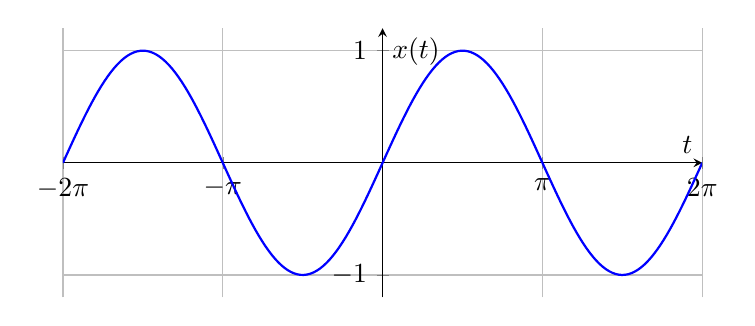
\begin{tikzpicture}
        \begin{axis}[
            width=0.8\textwidth,
            height=5cm,
            axis lines=middle,
            xlabel={$t$},
            ylabel={$x(t)$},
            domain=-2*pi:2*pi,
            samples=200,
            xtick={-6.2832,-3.1416,0,3.1416,6.2832},
            xticklabels={$-2\pi$,$-\pi$,$0$,$\pi$,$2\pi$},
            ytick={-1,0,1},
            ymin=-1.2, ymax=1.2,
            grid=both,
        ]
        \addplot[blue, thick] {sin(deg(x))};
        \end{axis}
    \end{tikzpicture}
    \caption{Verlauf der Sinusfunktion $x(t) = \sin(t)$ über zwei Perioden}
    \label{fig:sinus}
\end{figure}

Die Fourier-Transformierte der Sinusfunktion $x(t) = \sin(t)$ ist gegeben durch:
\[
\mathcal{F}\{\sin(\omega_0 t)\} = \pi j \left[ \delta(\omega + \omega_0) - \delta(\omega - \omega_0) \right]
\]
Für $\omega_0 = 1$ ergibt sich:
\[
\mathcal{F}\{\sin(t)\} = \pi j \left[ \delta(\omega + 1) - \delta(\omega - 1) \right]
\]
Der Betrag der Fourier-Transformierten besteht also aus zwei Dirac-Impulsen bei $\omega = \pm 1$.

Die graphische Darstellung der Fourier-Transformierten der Sinusfunktion ist in Abbildung \ref{fig:fourier_sinus_komplex} zu sehen.
\begin{figure}[H]
    \centering
    \begin{tikzpicture}
        \begin{axis}[
            width=0.8\textwidth,
            height=5cm,
            axis lines=middle,
            xlabel={$\omega$},
            ylabel={$\mathcal{F}\{\sin(\omega_0 t)\}$},
            xtick={-1,0,1},
            xticklabels={$-\omega_0$,$0$,$\omega_0$},
            ytick=\empty,
            ymin=-1.2, ymax=1.2,
            xmin=-1.5, xmax=1.5,
            grid=both,
            clip=false,
        ]
        % Dirac impulses: +1 at -omega0, -1 at +omega0
        \addplot+[ycomb, thick, blue, mark=*, samples at={-1}] {1};
        \addplot+[ycomb, thick, red, mark=*, samples at={1}] {-1};
        \node[above] at (axis cs:-1,1) {$\pi j\,\delta(\omega + \omega_0)$};
        \node[below] at (axis cs:1,-1) {$-\pi j\,\delta(\omega - \omega_0)$};
        \end{axis}
    \end{tikzpicture}
    \caption{Graphische Darstellung der Fourier-Transformierten der Sinusfunktion.}
    \label{fig:fourier_sinus_komplex}
\end{figure}

Die Sinusfunktion spielt eine immens wichtige Rolle in der digitalen Signalverarbeitung, da es der Grundstein der Fourier-Analyse (Fourier-Reihen und Fourier-Transformation) ist. Auch sind diese für lineare zeitinvariante Systeme (LTI) von Bedeutung. 
Der Sinus ist eine elementare periodische Funktion, seine Periodizität ist das grundlegende Konzept in vielen Signalen. Er lässt auch unter anderem komplex erscheinende Funktionen in Sinuskomponenten zerlegen und somit sie einfacher und kompakter darstellen.
Auch in der analogen Signalverarbeitung ist der Sinus von Bedeutung, da er die Basis für die Amplituden-, Frequenz- und Phasenmodulation bildet. Schließlich ist die Idealform der aus der Steckdose kommenden Netzspannung eine Sinuswelle, die in vielen Anwendungen als Referenzsignal dient. 

\subsection{Multiplikation der beiden Funktionen im Zeitbereich}
Bei einer Multiplikation der beiden Funktionen im Zeitbereich, also der Rechteckfunktion $x(t)$ und der Sinusfunktion $y(t)$, ergibt sich eine neue Funktion $z(t) =  x(t) \cdot y(t)$, die in Abbildung \ref{fig:rechteck_sinus} dargestellt ist. Diese Funktion ist das Ergebnis der Punkt-für-Punkt-Multiplikation der beiden Funktionen.
\begin{figure}[H]
    \centering
    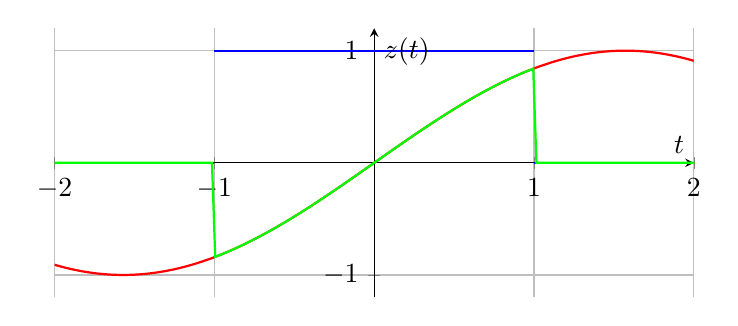
\begin{tikzpicture}
        \begin{axis}[
            width=0.8\textwidth,
            height=5cm,
            axis lines=middle,
            xlabel={$t$},
            ylabel={$z(t)$},
            domain=-2:2,
            samples=200,
            xtick={-2,-1,0,1,2},
            ytick={-1,0,1},
            ymin=-1.2, ymax=1.2,
            grid=both,
        ]
        % Rechteckfunktion
        \addplot[blue, thick, samples=2, domain=-2:-1] {0};
        \addplot[blue, thick, samples=2, domain=-1:1] {1};
        \addplot[blue, thick, samples=2, domain=1:2] {0};
        % Sinusfunktion
        \addplot[red, thick] {sin(deg(x))};
        % Multiplikation der beiden Funktionen
        \addplot[green, thick] {sin(deg(x)) * (x >= -1 && x <= 1)};
        \end{axis}
    \end{tikzpicture}
    \caption{Multiplikation der Rechteckfunktion $x(t)$ und der Sinusfunktion $y(t)$ im Zeitbereich}
    \label{fig:rechteck_sinus}
\end{figure}

Die Fourier-Transformierte der Multiplikation zweier Funktionen im Zeitbereich ist gegeben durch die Faltung ihrer Fourier-Transformierten im Frequenzbereich. Das bedeutet, dass die Fourier-Transformierte von $z(t)$, also $\mathcal{F}\{z(t)\}$, das Ergebnis der Faltung der Fourier-Transformierten von $x(t)$ und $y(t)$ ist:
\[
\mathcal{F}\{z(t)\} = \mathcal{F}\{x(t)\} * \mathcal{F}\{y(t)\}
\]

Es ergibt sich also eine neue Funktion im Frequenzbereich, die die Frequenzkomponenten der beiden ursprünglichen Funktionen kombiniert. Diese sieht folgendermaßen aus:
\begin{figure}[H]
    \centering
    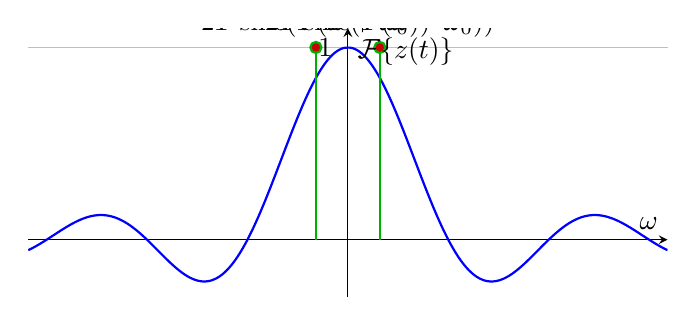
\begin{tikzpicture}
        \begin{axis}[
            width=0.8\textwidth,
            height=5cm,
            axis lines=middle,
            xlabel={$\omega$},
            ylabel={$\mathcal{F}\{z(t)\}$},
            domain=-10:10,
            samples=400,
            xtick=\empty, % entfernt die Zahlen auf der x-Achse
            ytick={-1,0,1},
            ymin=-0.3, ymax=1.1,
            grid=both,
        ]
        % Rechteckfunktion im Frequenzbereich
        \addplot[blue, thick, samples=400, domain=-10:10] {sin(deg(x))/x};
        % Sinusfunktion im Frequenzbereich (wird durch Dirac-Impulse dargestellt)
        % Faltung der beiden Funktionen im Frequenzbereich: Zwei Impulse bei -w_0 und w_0
        \addplot+[ycomb, thick, green!70!black, mark=*, samples at={-1,1}] {1};
        \node[above] at (axis cs:-1,1) {$2T\,\mathrm{sinc}(T(\omega+\omega_0))$};
        \node[above] at (axis cs:1,1) {$2T\,\mathrm{sinc}(T(\omega-\omega_0))$};
        \end{axis}
    \end{tikzpicture}
    \caption{Faltung der Fourier-Transformierten der Rechteckfunktion und der Sinusfunktion im Frequenzbereich}
    \label{fig:faltung_rechteck_sinus}
\end{figure}
\section{Zusammenhang von Datenrate und Bandbreite}
blabla
\clearpage